%!TEX root = ../3dbook.tex
% chktex-file 46

\setchapterpreamble[u]{\margintoc}

\graphicspath{{iso19107/}}
% \renewcommand*{\thelesson}{3.2}

\chapter{Three-dimensional geometries in geoinformation}%
\label{chap:iso19107}

To facilitate and encourage the exchange and interoperability of geographical information, the ISO (International Organization for Standardization: \url{www.iso.org}) and the OGC (Open Geospatial Consortium: \url{www.opengeospatial.org}) have developed in recent years standards that define what the basic geographical primitives are (the abstract specifications of ISO19107), and also how they can be represented in a computer (the implementation specifications of GML and \emph{Simple Features}). 
While the abstract definitions for the primitives are not restricted to two dimensions (2D), most of the efforts for the representation and storage of the geographical primitives have been done only in 2D; the \emph{Simple Features} specifications are well-defined, used, and implemented across the GIS community.
\marginnote{Simple Features specifications}\index{Simple Features specifications}

This document gives an overview of the primitives in 3D, both from the ISO19107 and the GML point-of-views.
Although the topic might appear trivial---``a polyhedron is simply a polyhedron, no?''---it is in practice a problem because several definitions exist and different software packages use different ones.
\marginnote{polyhedron}\index{polyhedron}

Having unambiguous definitions for the geometric primitives is important to foster interoperability, because most GIS operations (\eg\ calculation of the area of polygons; creation of buffers; conversion to other formats; Boolean operations such as intersection, union, etc.) require that the input primitives be according to certain definitions, otherwise the output of the operation is not guaranteed.

%%%
%
\section[Same polyhedra?]{Are your polyhedra the same as my polyhedra?}%
\label{sec:definition}

In the scientific literature, there is no single definition for a solid or a polyhedron (notice that these two terms are often used interchangeably).
Even in the field of mathematics, opinions differ as to what constitutes the term \emph{polyhedron}; many simply characterise the term as ``difficult to define''. 
Some researchers use it only for a regular polyhedron, or only for a convex one, and some consider non-planar faces as part of the definition.

%

The most common definition used is probably this simple one: a polyhedron is a 3D solid bounded by planar faces. 
The bounding faces are surfaces embedded in $\mathbb{R}^3$, the three-dimen\-si\-o\-nal Euclidean space, and together the bounding surfaces form a \emph{closed two-dimensional manifold} (or 2-manifold for short).
\marginnote{2-manifold}\index{2-manifold}
A 2-manifold is a topological space that is topologically equivalent to $\mathbb{R}^2$. 
An obvious example is the surface of the Earth, for which near to every point the surrounding area is topologically equivalent to a plane. 
An example of a 3-manifold is the entire Earth (its interior) because the neighbourhood of every point is equivalent to a sphere. 
\marginnote{3-manifold}\index{3-manifold}
The concept of neighbourhood, or locality, is such that a manifold can actually be constructed by `gluing' separate Euclidean spaces together.
Representing and storing a 2-manifold, even in $\mathbb{R}^3$, can be done with data structures that are intrinsically 2D since: (1) each edge is guaranteed to have a maximum of two incident faces; (2) around each vertex the incident faces form one `umbrella' (Figure~\ref{fig:nonmanifold}).
\begin{marginfigure}
  \centering
  \includegraphics[width=0.9\linewidth]{figs/nonmanifold}
  \caption{An example of an invalid 2-manifold: one edge and one vertex are non-manifold (the red ones).}%
\label{fig:nonmanifold}
\end{marginfigure}
The 2D data structures typically used in GIS, \eg\ the half-edge or the DCEL, can thus be used.



%%%
%
\section{The standard ISO19107}

The geometric primitives as used in 3D GIS are based on the ISO19107 definitions, and the definition of a polyhedra there is broader than that of a 2-manifold, to allow us to represent all the real-world features.

As shown in Figure~\ref{fig:isoprimitives}, 
\begin{marginfigure}
  \centering
  \includegraphics[width=\linewidth]{figs/isoprimitives.pdf}
  \caption{ISO 19017 primitives relevant for the modelling of the built environment.}%
\label{fig:isoprimitives}
\end{marginfigure}
the ISO19107 geometric primitives for representing an object are: a 0D primitive is a \texttt{GM\_Point}, a 1D a \texttt{GM\_Curve}, a 2D a \texttt{GM\_Surface}, and a 3D a \texttt{GM\_Solid}.
A $d$-dimensional primitive is built with a set of $(d-1)$-dimensional primitives, \eg\ a \texttt{GM\_Solid} is formed by several \texttt{GM\_Surfaces}, which are formed of several \texttt{GM\_Curves}, which are themselves formed of \texttt{GM\_Point}.
Observe that the ISO19107 primitives do not need to be linear or planar, \ie\ curves defined by mathematical functions are allowed

%

In our context, the following three definitions from \citet{ISO19107} are relevant:
\begin{definition}
A \texttt{GM\_Solid} is the basis for 3-dimensional geometry. 
The extent of a solid is defined by the boundary surfaces.
The boundaries of \texttt{GM\_Solids} shall be represented as \texttt{GM\_SolidBoundary}.
[\ldots] 
The \texttt{GM\_OrientablesSurfaces} that bound a solid shall be oriented outward.
\end{definition}
\begin{definition}
A \texttt{GM\_Shell} is used to represent a single connected component of a \texttt{GM\_SolidBoundary}. 
It consists of a number of references to \texttt{GM\_OrientableSurfaces} connected in a topological cycle (an object whose boundary is empty). 
[\ldots] 
Like \texttt{GM\_Rings}, \texttt{GM\_Shells} are simple.
\end{definition}
\begin{definition}
A \texttt{GM\_Object} is \emph{simple} if it has no interior point of self-intersection or self-tangency. 
In mathematical formalisms, this means that every point in the interior of the object must have a metric neighbourhood whose intersection with the object is isomorphic to an $n$-sphere, where $n$ is the dimension of this \texttt{GM\_Object}.
\end{definition}

%

Observe that since shells (\texttt{GM\_Shell}s) are \emph{simple}, they are 2-manifold objects.
To be a valid shell, the 2-manifold should be closed, \ie\ there should not be `holes' in the surface (in other words, it should be watertight).
% It should furthermore be an orientable surface, Möbius strip not allowed.
% From Claus Nagel: However, the shell of a solid cannot be any 2-manifold, it must be a closed, orientable surface. Specifically, the shell must be homeomorphic to an n-holed torus, with the 0-holed torus being the n-sphere.

%

Figure~\ref{fig:onesolid} shows a solid that respects that definition.
\begin{marginfigure}
  \centering
  \includegraphics[width=0.95\textwidth]{figs/isosolid.pdf}
  \caption{One solid which respects the ISO19107 definition. It has one exterior shell (grey) and one interior shell (orange) forming a cavity.}%
\label{fig:onesolid}
\end{marginfigure}
First observe that the solid is composed of two shells (both forming its boundaries), one being the exterior and one being the interior shell.
The exterior shell has eleven surfaces, and the interior one six.
An interior shell creates a cavity in the solid---cavities are also referred to as ``voids'' or holes in a solid.
A solid can have no inner shells, or several.
Observe that a cavity is not the same as a hole in a torus (a doughnut) such as that in Figure~\ref{fig:torus}: it can be represented with one exterior shell having a genus of 1\marginnote{The \textbf{genus} of an (orientable) surface embedded is the number of ``handles'' that it has. For instance, a doughnut and a mug have a genus of 1.} and no interior shell.
Observe also that the top face of the solid in Figure~\ref{fig:onesolid} has one inner ring, but that other surfaces ``fill'' that hole so that the exterior shell is closed.
\begin{marginfigure}
  \centering
  \includegraphics[width=0.8\linewidth]{figs/torus.pdf}
  \caption{A `squared torus' is modelled with one exterior boundary formed of ten surfaces. Notice that there are no interior boundary.}%
\label{fig:torus}
\end{marginfigure}


%%%
%
\section{Primitives used in practice}

\begin{figure}
  \centering
  \includegraphics[width=0.7\linewidth]{figs/geomprimitives.pdf}
  \caption{Some of the CityGML primitives, including aggregates and composites. Orange primitives are those representing inner boundaries. The \texttt{Shell} is not a class in GML, but it is implied when a \texttt{CompositeSurface} is used to define the boundary of a \texttt{Solid}.}%
\label{fig:geomprimitives}
\end{figure}

%

CityGML, the international standard for 3D modelling of cities (see Chapter~\ref{chap:3dcm}), uses a subset of ISO19107, with the following two restrictions: 
\begin{enumerate}
  \item \texttt{GM\_Curves} can only be \emph{linear} (thus only \texttt{LineStrings} and \texttt{LinearRings} are used); 
  \item \texttt{GM\_Surfaces} can only be \emph{planar} (thus \texttt{Polygons} are used).
\end{enumerate}

%

Following ISO19107, in GML and CityGML geometric primitives can be combined into either \emph{aggregates} or \emph{composites}.

An aggregate (class \texttt{gml:\_AbstractGeometricAggregate}) is an arbitrary collection of primitives of same dimensionality that is simply used to bundle together geometries.
GML (and CityGML) has classes for each dimensionality (\texttt{Multi*}), the most relevant one in our context is \texttt{MultiSurface} that is often used in practice to represent the geometry of a building.
An aggregate does not prescribe any topological relationships between the primitives.

A composite of dimension $d$ is a collection of $d$-dimensional primitives that form a $d$-manifold. 
\marginnote{$d$-manifold}\index{$d$-manifold}
The most relevant example in our context is a \texttt{CompositeSurface}, which is a 2-manifold.



%%%
%
\section[Implementation specifications]{Implementation specifications for the 3D primitives}


Observe that for a primitive to be valid, all its lower-dimensionality primitives have to be valid.
For instance, a valid Solid cannot have as one of its surfaces a Polygon having a self-intersection (which would make it invalid).


%%%
\subsection{\texttt{Polygon}}

For a \texttt{Polygon} embedded in $\mathbb{R}^3$ to be valid, it needs to fulfil the 6 assertions in Figure~\ref{fig:ogcsf_definitions}, which are given on pages 27--28 of the OGC \emph{Simple Features} document.
These rules are verified by first projecting each \texttt{Polygon} to a plane, this plane is usually obtained by least-square adjustment of its points.
A \texttt{Polygon} must also be \emph{planar} to be valid: its points (used for both the exterior and interior rings) have to lie on a plane.
\begin{figure}
  \centering
  \begin{boxedminipage}{\textwidth}
    {\small
  \begin{enumerate}
    \item Polygons are topologically closed;
    \item The boundary of a Polygon consists of a set of LinearRings that make up its exterior and interior boundaries;
    \item No two Rings in the boundary cross and the Rings in the boundary of a Polygon may intersect at a Point but only as a tangent, \eg\
      \[
         \forall P \in Polygon, \forall c1, c2 \in P.Boundary(), c1 \neq c2,
      \]
      \[
          \forall p, q \in Point, p, q \in c1, p \neq q, [p \in c2 \Rightarrow q \notin c2];
      \]
    \item A Polygon may not have cut lines, spikes or punctures \eg:
      \[
         \forall P \in Polygon, P = P.Interior.Closure;
      \]
    \item The interior of every Polygon is a connected point set;
    \item The exterior of a Polygon with 1 or more holes is not connected. Each hole defines a connected component of the exterior.
  \end{enumerate}
  }
  \end{boxedminipage}
\caption{The six assertions for the validity of a 2D polygon, according to \emph{Simple Features}.}%
\label{fig:ogcsf_definitions}
\end{figure}



%%%
\subsection{\texttt{MultiSurface}}
It is an arbitrary collection of \texttt{Polygon}.
Validating a \texttt{MultiSurface} simply means that each \texttt{Polygon} is validated individually; a \texttt{MultiSurface} is valid if all its \texttt{Polygon}s are valid.


%%%
\subsection{\texttt{CompositeSurface}}
Besides that each \texttt{Polygon} must be individually valid, the \texttt{Polygon}s forming a \texttt{Composite\-Surface} are not allowed to overlap and/or to be disjoint.
Furthermore, if we store a \texttt{Com\-po\-site\-Surface} in a data structure, each edge is guaranteed to have a maximum of two incident surfaces (except those on the boundary), and around each vertex the incident faces form one ``umbrella'' (see Figure~\ref{fig:nonmanifold}).


%%%
\subsection{\texttt{Solid}}

According to ISO19107, the different boundaries of a solid are allowed to interact with each other, but only under certain circumstances.
To understand these, we have to generalise to 3D the implementation specifications defined in 2D by the OGC (Figure~\ref{fig:ogcsf_definitions}).
Observe that all of them, except the third one, generalise directly to 3D since a point-set topology nomenclature is used.
The only modifications needed are that, in 3D, polygons become solids, rings become shells, and holes become cavities.

To further explain what the assertions are in 3D, Figure~\ref{fig:validornot}
\begin{figure}
  \centering
  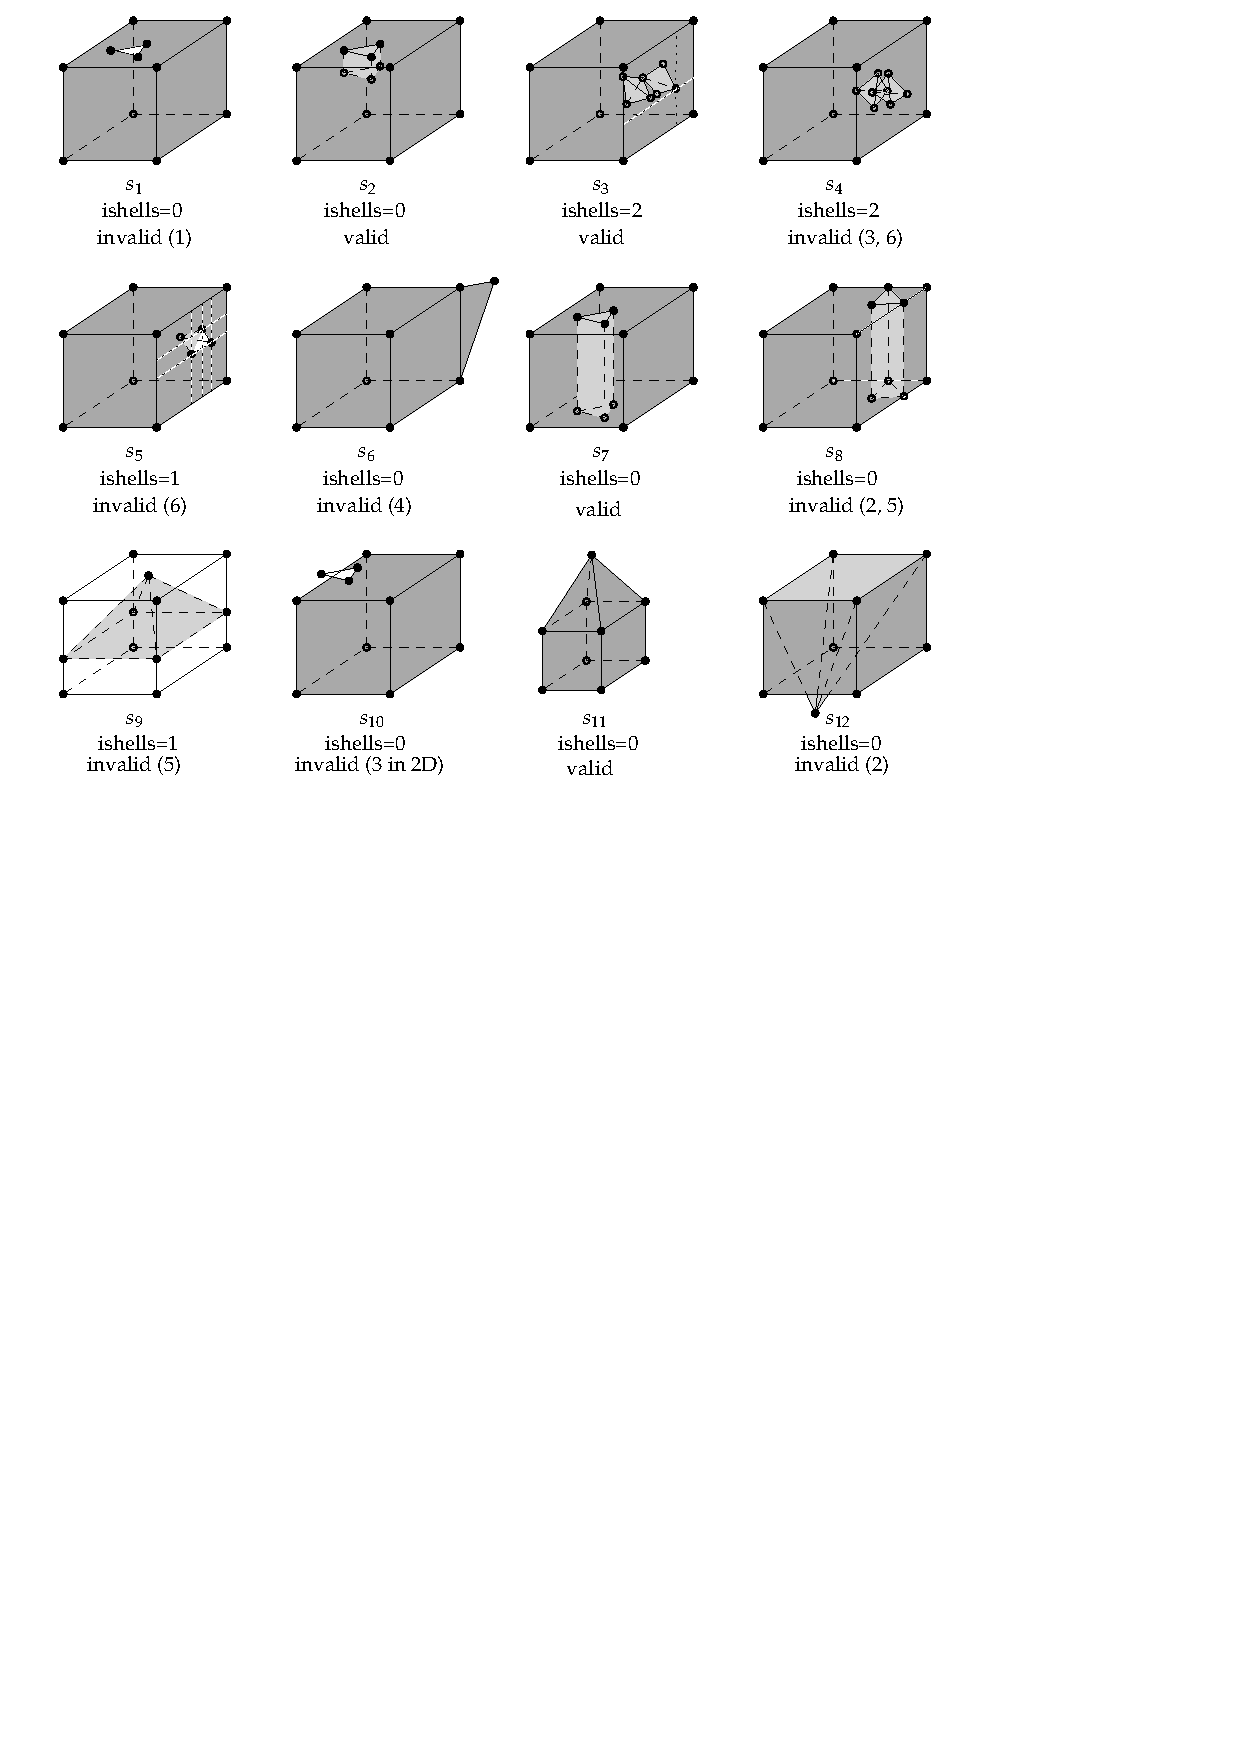
\includegraphics[width=\textwidth]{figs/validornot.pdf}
  \caption{Twelve solids, some of them valid some invalid. The number of interior shell(s) is ``ishell'', and the numbers in parentheses next to invalid indicates which OGC assertions are broken. For solid $s_9$ the colour of the exterior shell is not shown to highlight the interior shell.}%
\label{fig:validornot}
\end{figure}
shows 12 solids, some of them valid, some not (all the statements below refer to solids in this figure).

The first assertion of the OGC means that a solid must be closed, or `watertight' (even if it contains interior shells).
The solid $s_1$ is thus not valid, but $s_2$ is because the hole in the top surface is `filled' with other faces.

The second assertion implies that each shell must be simple, \ie\ that it is a 2-manifold.

The third assertion means that the boundaries of shells can intersect each others, but the intersection between the shells can only contain primitives of dimensionality 0 (vertices) and 1 (edges).
If a surface or a volume is part of the intersection, then the solid is invalid.
The solid $s_3$ is an example of a valid solid: it has two interior shells whose boundaries intersect at one point (at the apexes of the tetrahedra), and the apex of one of the tetrahedra is coplanar with the exterior shell.
If the interior of the two interior shells intersects (as in $s_4$) the solid is not valid; this is also related to the sixth assertion stating that each cavity must define one connected component: if the interior of two cavities are intersecting they define the same connected component.
Notice also that $s_5$ is not valid since one surface of its cavity intersects with one surface of the exterior shell (they ``share a surface''); $s_5$ should be represented with one single exterior shell (having a `dent'), and no interior shell.

The fourth assertion states that a shell is a 2-manifold and that no dangling pieces can exist (such as that of $s_6$); it is equivalent to the \emph{regularisation} of a point-set in $\mathbb{R}^3$.
\marginnote{regularisation}\index{regularisation}

The fifth assertion states that the interior of a solid must form a connected point-set (in $\mathbb{R}^3$).
Consider the solid $s_7$, it is valid since its interior is connected and it fulfils the other assertions; notice that: (1) it is a 2-manifold but that unlike other solids in Figure~\ref{fig:validornot} (except $s_8$) its genus is 1; (2) it is modelled only with an exterior shell.
If we move the location of the triangular prism (which is part of the exterior shell, and is not an interior shell) so that it touches the boundary of the exterior shell (as in $s_8$), then the solid becomes invalid since its interior is not connected anymore, and also since its exterior shell is not simple anymore (2 edges have 4 incident planar faces, which is not 2-manifold).
It is also possible that the interior shell of a solid separates the solid into two parts: the interior shell of $s_9$ is a pyramid having four of its edges intersecting with the exterior shell, but no two surfaces are shared, thus these interactions are allowed.
However, the presence of the pyramid separates the interior of the solid into two unconnected volumes (violating assertion 5); for both $s_8$ and $s_9$, the only possible valid representation is with two different solids.

Notice also that for a solid to be valid, all its lower-dimensionality primitives must be valid.
That is, each surface of the shells has to be individually valid according to the assertions in Figure~\ref{fig:ogcsf_definitions}.
An example of an invalid surface would be one having a hole (an inner ring) overlapping the exterior ring (see $s_{10}$).

It should also be noticed that when validating a solid both the combinatorial consistency and the geometric consistency of the representation should be valid.
\marginnote{combinatorial consistency}\index{combinatorial consistency}
A solid such as $s_{11}$ is valid, but if the location of only one of its vertices is modified (for instance if the apex of the pyramid of $s_{11}$ is moved downwards to form $s_{12}$) then it becomes invalid. 
Both $s_{11}$ and $s_{12}$ can be represented with a graph having exactly the same topology (which is valid for both), but if we consider the geometry then the latter solid is not valid since its exterior shell is not simple.
Enforcing simplicity requires calculating the intersections between the surfaces.

Lastly, the orientation of the polygons must be considered.
In 2D, the only requirement for a polygon is that its exterior ring must have the opposite orientation of that of its interior ring(s) (\eg\ clockwise versus counter-clockwise).
In 3D, if one polygon is used to construct a shell, its exterior ring must be oriented in such as way that when viewed from outside the shell the points are ordered counter-clockwise.
Figure~\ref{fig:orientation} shows an example.
\begin{marginfigure}
  \centering
  \includegraphics[width=0.8\linewidth]{figs/orientation.pdf}
  \caption{One solid and the orientation of 3 of its polygons (different colours).}%
\label{fig:orientation}
\end{marginfigure}
In other words, the normal of the surface must point outwards if a right-hand system is used, \ie\ when the ordering of points follows the direction of rotation of the curled fingers of the right hand, then the thumb points towards the outside.
If the polygon has interior rings, then these have to be ordered clockwise.


\begin{kaobox}[frametitle=\faCog\ How does it work in practice?]
  The software `val3dity', developed at TU Delft, allows us to validate directly all the ISO19107 primitives, it accepts as input CityJSON and OBJ, among others.
  It is freely available at \url{https://github.com/tudelft3d/val3dity}, and a web-application can be used at \url{http://geovalidation.bk.tudelft.nl/val3dity/}
\end{kaobox}

%%%
\subsection{\texttt{MultiSolid}}
It is an arbitrary collection of \texttt{Solid}s.
Validating a \texttt{MultiSolid} simply means that each \texttt{Solid} is validated individually; a \texttt{MultiSolid} is valid if all its \texttt{Solid}s are valid.


%%%
\subsection{\texttt{CompositeSolid}}
A \texttt{CompositeSolid}, formed by the \texttt{Solids} $A$ and $B$, should fulfil the following two assertions:
\begin{itemize}
  \item \textbf{Assertion \#1:} their interior should not overlap ($A^{o} \cap B^{o} = \emptyset$)
  \item \textbf{Assertion \#2:} their union should form one solid ($A \cup B =$ one \texttt{Solid})
\end{itemize}


%%%
%
\section{Notes and comments}

The title ``\emph{Are your polyhedra the same as my polyhedra?}'' is taken from the (excellent) paper from \citet{Grunbaum03}.

The 2D GIS data structures that can be used for storing 2-manifolds are, for instance, the half-edge~\citep{Mantyla88}, the quad-edge~\citep{Guibas85}, and the doubly-connected edge list (DCEL)~\citep{Muller78}; all of these store the edge of a polyhedron as the atom, with links to its adjacent edges and incident faces.

For details how the validation of a the 3D primitives can be implemented, see \citet{13_cacaie} and \citet{18_ogdss_val3dity}.

The official specifications documents are the following:
\begin{itemize}
  \item ISO19107 document: \citet{ISO19107}
  \item Simple Features document: \citet{OGC-SF}
  \item GML specifications: \citet{OGC-GML}
  \item CityGML specifications: \citet{CityGML3.0CM}
\end{itemize}


%%%
%
\section{Exercises}

\begin{enumerate}
  \item List all 10 surfaces (and describe their geometry) for the solid in Figure~\ref{fig:torus}.
  \item Draw a 2-manifold that has a genus of 2.
  \item The object in Figure~\ref{fig:nonmanifold} contains 8 surfaces but is not a 2-manifold. If you were to store it in a 3D primitive in GML, which one would you choose? 
  \item How many interior shells does the solid in Figure~\ref{fig:orientation} have?
  \item In which direction points the normal of the interior shell of the solid in Figure~\ref{fig:geomprimitives}?
\end{enumerate}
